\chapter{Wykład 14. Zarządzanie ryzykiem w projekcie informatycznym}

\section{Macierz ryzyka}
% strona 27

Ten wirtualny warsztat jest beznadziejny.

% ===========================================================================

\section{Rejestr ryzyka projektowego}
% strona 36

Ten wirtualny warsztat jest beznadziejny.

% ===========================================================================

\section{Analiza jakościowa i ilościowa SWOT}
% strona 48

\begin{figure}[h]
\begin{center}
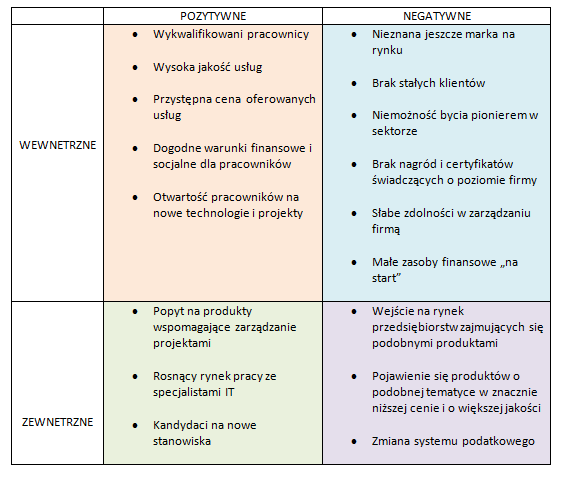
\includegraphics[scale=1]{swot.png}
\caption[Analiza SWOT]{Analiza SWOT}
\label{rysunekProces}
\end{center}
\end{figure}

\clearpage

% ===========================================================================

\section{Analiza jakościowa ryzyka}
% strona 54

Na pół roku przed końcem projektu, inwestor wycofuje się z projektu, zarzucając go.
\begin{itemize}
\item zgodnie z zapisem w umowie otrzymujemy 200 000 tys zł odszkodowania, za zerwanie umowy
\item postanawiamy dokończyć projekt w przeciągu pół roku, a następnie znaleźć chętnych na niego klientów
\item PMBOK jest popularny, więc powinniśmy znaleźć przedsiębiorstwo które pracuje zgodnie z nim
\item Zarzucenie projektu, który jest w wysokim stopniu zaawansowania prac jest nieopłacalne
\end{itemize}

Prawdopodobieństwo:  M - małe, S – średnie, D – duże\\
Wpływ: N - niski, P – poważny, W – wielki

\begin{table}[htb]
\centering
\begin{tabular}{c|p{11.5cm}|c|c} 
Lp. & Opis & Prawdop. & Wpływ \\
 \hline 1 & Zbyt długi czas realizacji projektu & S & P \\
 2 & Skończenie się środków z odszkodowania które zostały przeznaczone na projekt & S & W \\
 3 & Niemożliwość znalezienia kupca chętnego na projekt po jego zakończeniu & M & W \\
 4 & Odejście przed zakończeniem projektu, któregoś z członków grupy projektowej & M & W \\
5 & Długotrwała choroba kogoś z grupy projektowej & S & P \\
6 & Otrzymanie innego dużego zlecenia w trakcie prac nad dokończeniem projektu & S & N \\
7 & Przedłużający się proces z inwestorem w sprawie odszkodowania & D & P \\
8 & Ukazanie się we wcześniejszym terminie produktu konkurencyjnej firmy & M & P \\
9 & Wewnętrzna sytuacja w firmie zmuszająca do przeznaczenia środków z odszkodowania na inne cele  & M & P  \\
10 & Pomimo znalezienia klientów inwestycja nie zwraca się &  S & N  \\
\end{tabular}
\caption{\textbf{Analiza jakościowa ryzyka}}
\label{tab:analizaJakosciowa}
\end{table}

\clearpage

\begin{table}[!h]
\centering
\begin{tabular}{c|c|c|c} Prawdop. \textbackslash Wpływ & Niski & Poważny & Wielki \\
 \hline Duże &  & 7 &  \\
 Średnie & 6,10 & 1,5 & 2 \\
 Małe &  & 8,9  & 3,4  \\
\end{tabular}
\caption{\textbf{Macierz prawdopodobieństwa}}
\label{tab:macierzPrawdopodobienstwa}
\end{table}




% ===========================================================================

\section{Analiza ilościowa ryzyka}
% strona 62

Ten wirtualny warsztat jest beznadziejny.

% ===========================================================================

\section{Plany reakcji na ryzyko}
% strona 75

\begin{figure}[h]
\begin{center}
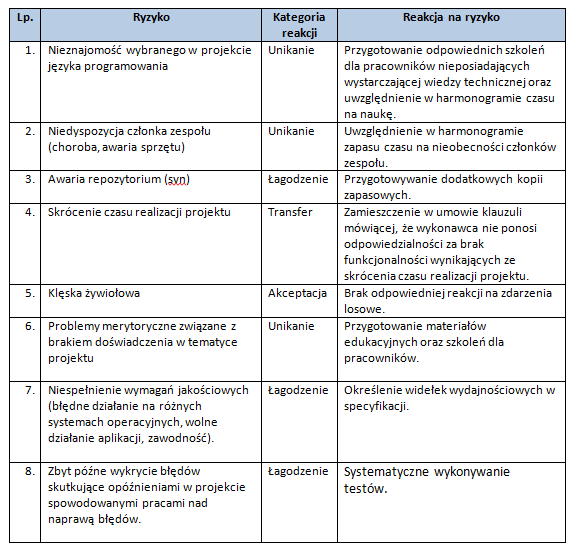
\includegraphics[scale=1]{planreakcji.png}
\caption[Plan reakcji na ryzyko]{Plan reakcji na ryzyko}
\label{rysunekProces}
\end{center}
\end{figure}


